\section{Introdução}
    \label{sec:intro}
A percepção sobre o mundo é feita através dos sentidos, dentre eles existe a visão. Com ela a humanidade pode distinguir formas, padrões, luzes e sombras de estruturas 3D que a cerca. Ao possibilitar esta mesma interpretação ao computador têm-se a denominada~\emph{visão computacional}~\citep{Szeliski2012}. Esta área possui diversas aplicações, como:~\emph{autentificação visual},~\emph{geração de panorâmicas},~\emph{captura de movimentos},~\emph{vigilância},~\emph{modelagem 3D a partir de imagens} e tantas outras mais. Para os casos cujo objetivo é entender o mundo a partir das múltiplas imagens é preciso usar~\emph{visão estéreo}.

\subsection{Geometria}
    \label{subsec:intro_geo}
No sistema de coordenadas euclidianas há um problema da representatividade da origem e dos demais pontos, uma vez que o primeiro é um ponto distinto e os demais são geometricamente idênticos. Como solução têm-se as~\emph{coordenadas homogêneas}, onde a origem é removida do plano e acrescida de uma dimensão~\cite{Li2001}. Nestas coordenadas, têm-se as equivalências de representação: pontos 2D são representados como $\mathbf{X} = (x, y)$ no espaço euclidiano são representados como $\mathbf{\Tilde{X}} = \mathbf{\Tilde{w}}(x, y, 1)$; linha 2D de $\mathbf{L} = ax + by + c$ paraa $\mathbf{\Tilde{L}} = (a, b, c)$; e ponto 3D de $\mathbf{X} = (x, y, z)$ para $\mathbf{\Tilde{X}} = \mathbf{\Tilde{w}}(x, y, z, 1)$.

Em coordenadas homogêneas, as transformações geométricas são multiplicação de matrizes, como: a~\emph{translação} ($\mathbf{x}'_{trans} = \big[ ~\mathbf{I}  ~|~ \mathbf{t}~ \big] ~ \mathbf{\Tilde{x}}$) e a~\emph{rotação com translação} ($\mathbf{x}'_{rot + trans} = \big[ ~\mathbf{R}  ~|~ \mathbf{t}~ \big] ~ \mathbf{\Tilde{x}}$), onde $\mathbf{R}\mathbf{R}^{T} = \mathbf{I}$ e $| \mathbf{R} | = 1$.

Além disso, um produto vetorial $\mathbf{v}_{\times} = \mathbf{a} \times \mathbf{b}$ é equivalente à multiplicação de matrizes $\mathbf{v}_{\times} = {[\mathbf{a}]}_{\times} \mathbf{b}$, sendo ${[\mathbf{a}]}_{\times}$ a forma matricial do operador de produto vetorial~\cite{Szeliski2012}.

\subsection{Câmeras}
    \label{subsec:intro_cam}
Para a aquisição de imagens, uma câmera é posicionada no mundo com um ponto de referência
% , conforme ilustrado na Figura~\ref{fig:intro_cam_coord}
. Dessa forma, por semelhança de triângulos, a projeção $\mathbf{P}$ de pontos 3D do mundo em pontos 2D da imagem corresponde a $(x, y, z) \to (f \frac{X}{Z}, f \frac{Y}{Z}, f) = (f \frac{X}{Z}, f \frac{Y}{Z})$, ou seja, $\mathbf{P} \mathbf{X} = \mathbf{x}$.

% \begin{figure*}[!ht]
%     \begin{center}
%         \bmvaHangBox{\fbox{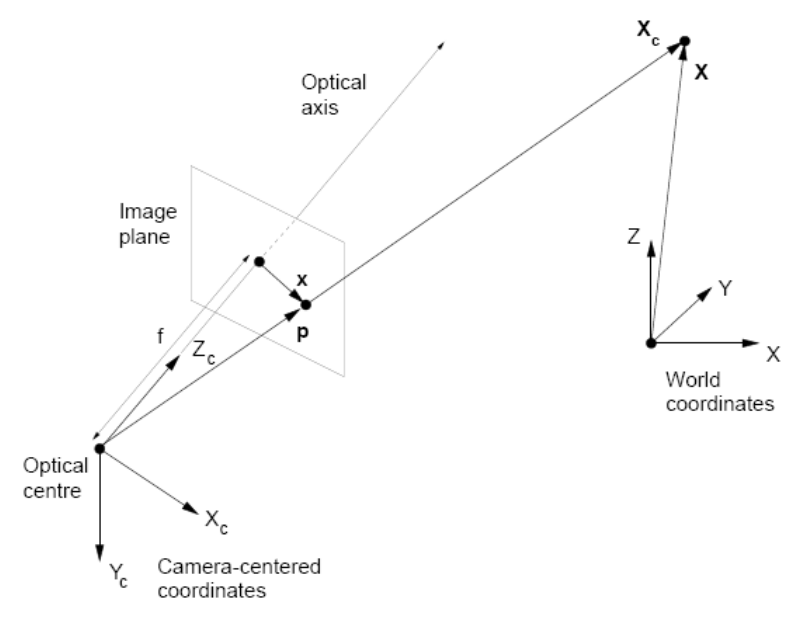
\includegraphics[width=5cm]{Figs/Introducao/cam_coord.png}}}
%     \end{center}
%     \caption{Localização e relação das coordenadas da câmera com a do mundo. Fonte~\cite{FergusL1}.}
%     \label{fig:intro_cam_coord}
% \end{figure*}

A projeção $\mathbf{P}$ é a combinação de três transformações de coordenadas:~\emph{matriz de intrínsecos} $\mathbf{K}$ (posicionamento do ponto focal e do ponto principal, ângulo entre eixos e outros), matriz de projeção $[\mathbf{I} ~|~ \mathbf{0} ]$ e~\emph{matriz de extrínsecos} $[\mathbf{R} ~|~ \mathbf{t} ]$ (relação entre as coordenadas da câmera e os~\emph{pixels})~\cite{FergusL1}.

% , onde:
% $$
%     {\mathbf{K}}
%     =
%     \begin{bmatrix} 
%         f_x & \alpha & c_x\\
%         0 & f_y & c_y \\
%         0 & 0 & 1 \\
%     \end{bmatrix}
%     =
%     \begin{bmatrix} 
%         \text{dist. focal em~\emph{pixels} hor.} & \text{âng. entre eixos} & \text{centro hor.} \\
%         0 & \text{dist. focal em~\emph{pixels} ver.} & \text{centro ver.} \\
%         0 & 0 & 1 \\
%     \end{bmatrix}
%     .
% $$

\subsection{Visão Estéreo}
    \label{subsec:intro_stereo}
A partir de duas ou mais imagens de um mesmo local (objeto ou até uma pessoa), é possível extrair, identificar e triangular suas características nas imagens e obter uma modelagem 3D; os problemas de~\emph{correspondência}~\cite{FergusL1}.

A priori a busca pelas correspondências ocorreria por toda a imagem; com uso das~\emph{linhas epipolares} reduz-se a uma busca linear. 
% Com base na Figura~\ref{fig:intro_stereo_epipolar_exemplo}, sabe-se
Sabe-se
que o ponto real $\mathbf{p}$ é representado pelos pontos $\mathbf{x_0}$ e $\mathbf{x_1}$ das imagens. Ao reprojetar linearmente o ponto $\mathbf{p}$ no infinito, $\mathbf{p_{\infty}}$, de modo a continuar sendo projetado no ponto $\mathbf{x_0}$ é possível determinar a linha epipolar a partir da diferença de projeção em relação a $\mathbf{x_1}$~\cite{Szeliski2012}.

% \begin{figure*}[!ht]
%     \begin{center}
%         \bmvaHangBox{\fbox{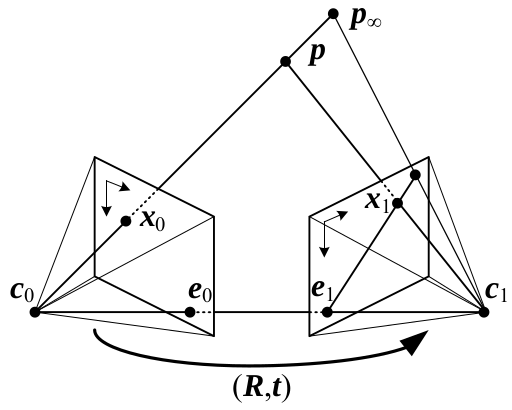
\includegraphics[width=3.8cm]{Figs/Introducao/linha_epipolar.png}}}
%     \end{center}
%     \caption{Representação visual da determinação de uma linha epipolar. Fonte~\cite{Szeliski2012}.}
%     \label{fig:intro_stereo_epipolar_exemplo}
% \end{figure*}

Com a aquisição das linhas epipolares de imagens correspondentes é possível reduzir a busca de correspondência numa linha horizontal, para alguns conjuntos de imagem~\cite{Szeliski2012}, 
% conforme ilustrado na Figura~\ref{fig:intro_stereo_match},
sendo denominado de~\emph{retificação}.

% \begin{figure}[!ht]
%     \centering
%     \begin{tabular}{cc}
%         \bmvaHangBox{\fbox{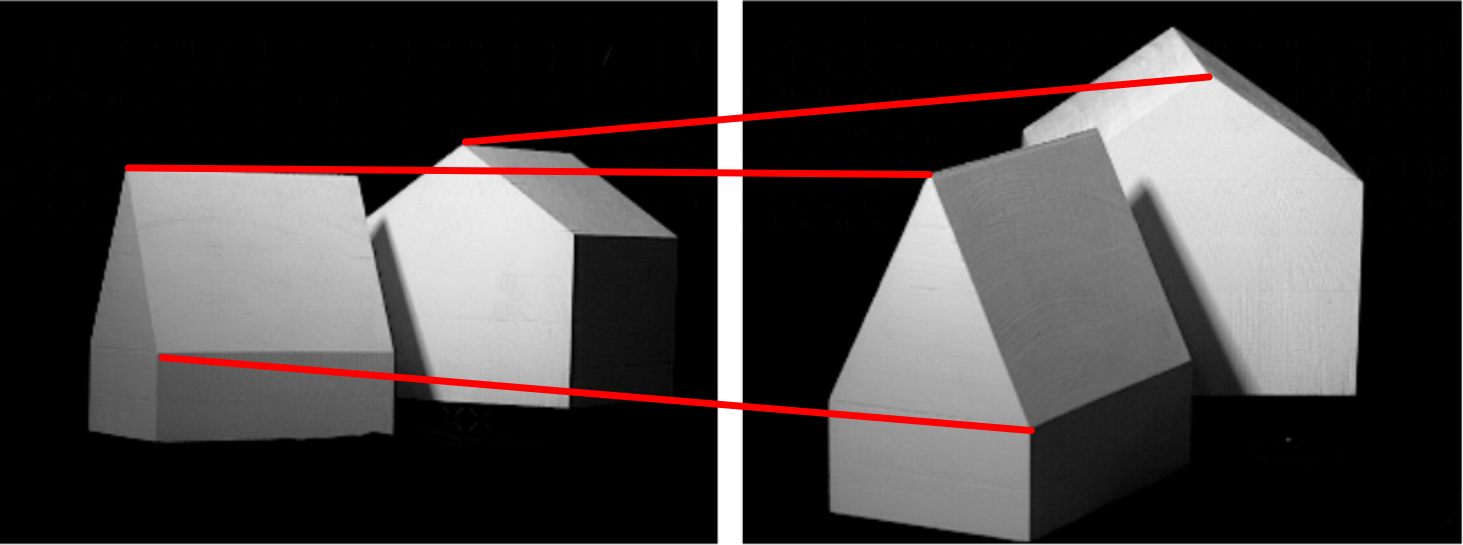
\includegraphics[height=1.5cm]{Figs/Introducao/original_stereo_.png}}}&
%         \bmvaHangBox{\fbox{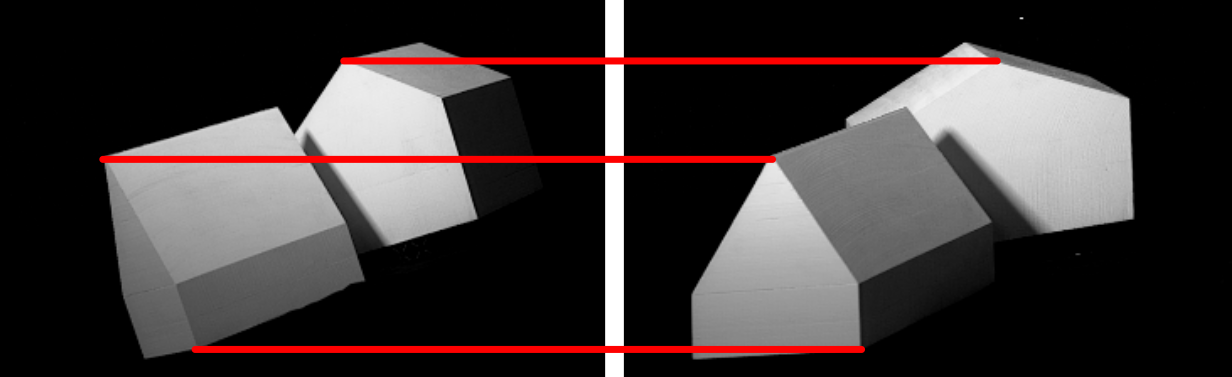
\includegraphics[height=1.5cm]{Figs/Introducao/ret_stereo_.png}}}\\
%         (a)&(b)
%     \end{tabular}
%     \caption{Retificação de um par de imagens estéreo, onde (a) são as imagens originais com linhas epipolares em diversas direções e (b) são as imagens retificação com todas as linhas epipolares na horizontal. Adaptado~\cite{Lazebnik1}.}
%     \label{fig:intro_stereo_match}
% \end{figure}

Além disso, a partir de duas imagens correspondentes a quantidade de movimentação que é percebida é denominada~\emph{disparidade}. Essa grandeza informa a distância entre os~\emph{pixels} correspondentes das imagens: $d_{(x, y)} = |x - x'| + |y - y'|$. Ao se calcular a disparidade para todos os~\emph{pixels} da imagem obtém-se seu~\emph{mapa de disparidade}
% , conforme ilustrado na Figura~\ref{fig:intro_stereo_disp_exemplo}
. No cenário de imagens correspondentes retificadas onde uma está certamente à direita da outra, a busca é ainda reduzida à esquerda do~\emph{pixel} base e vice-versa.

% \begin{figure}[!ht]
%     \centering
%     \begin{tabular}{cccc}
%         \bmvaHangBox{\fbox{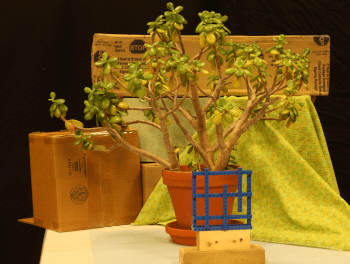
\includegraphics[width=3.3cm]{Figs/Introducao/exemplo_left.png}}}&
%         \bmvaHangBox{\fbox{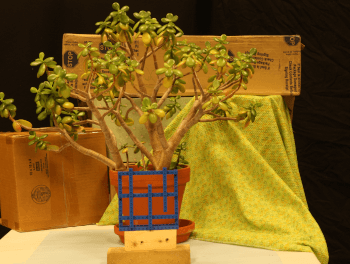
\includegraphics[width=3.3cm]{Figs/Introducao/exemplo_right.png}}}&
%         \bmvaHangBox{\fbox{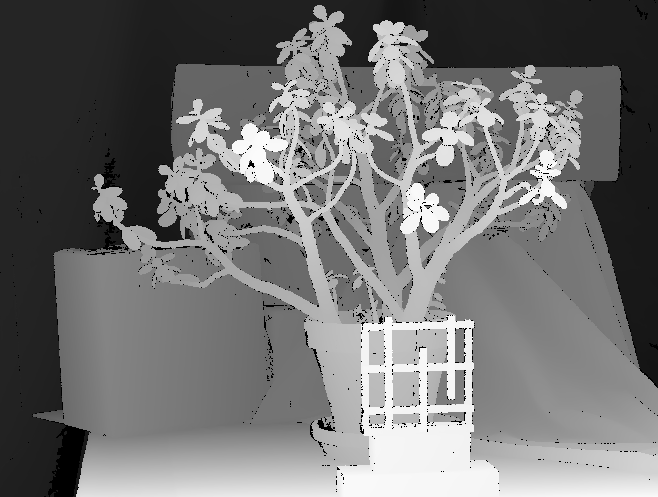
\includegraphics[width=3.3cm]{Figs/Introducao/exemplo_gt.png}}}\\
%         (a)&(b)&(c)
%     \end{tabular}
%     \caption{Mapa de disparidade para um par de imagens correspondentes retificadas, com as imagens exploradas por este trabalho. Têm-se os três componentes para esse mapa: (a) imagem base, (b) imagem correspondente à imagem base e (c) mapa de disparidade da imagem base.}
%     \label{fig:intro_stereo_disp_exemplo}
% \end{figure}

Com a aquisição do mapa de disparidade e em pose dos dados das câmeras (distância focal da imagem base $f$ e distância do mundo entre as câmeras $b$) é possível calcular o~\emph{mapa de profundidade}, uma vez que $Z_{xy} = (f \cdot b) /d_{xy}$.